\documentclass[12pt,letterpaper,titlepage]{article}

\usepackage{fontspec}
\defaultfontfeatures{Mapping=tex-text}
\usepackage{xunicode}
\usepackage{xltxtra}
\usepackage{amsmath}
\usepackage{pdfpages}
\usepackage{amsfonts}
\usepackage{bbold}
\usepackage{amssymb}
\setcounter{secnumdepth}{0}
\usepackage{nameref}
\usepackage{enumitem}
\usepackage{environ}
\usepackage{pgfplots}
\usepackage{listings}

\showboxdepth=\maxdimen
\showboxbreadth=\maxdimen


\usepackage{paracol}
\usepackage{wrapfig}
\globalcounter{table}
\globalcounter{figure}
\usepackage{graphicx}
\usepackage[left=1in,right=1in,top=1in,bottom=1in]{geometry}
\graphicspath{{img/}}

\author{Jacob Abel}
\title{	Design \& Simulate 8
	\\\large ECE2204 CRN:82929
}

\setlength{\parskip}{0.5em}

\begin{document}
\maketitle
\begin{raggedright}

\section{Problem 8.2-11.a.1: } The circuit was a random circuit I threw together in LTSpice.
\subsection{Design}
Using the circuit displayed below, determine the current flowing through $D_1$, $D_2$, $D_3$ and the voltage at points A, B, C, and D. Assume $V_\gamma = 0.5V$.

\begin{center}
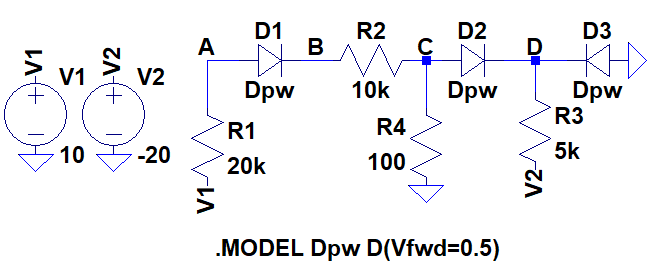
\includegraphics[width=\textwidth, height=9\baselineskip, keepaspectratio=true]{ds1}
\end{center}

Assume all diodes are on.

$V_D = -0.5$ $V_A = 10V$, and $V_B = V_C = 0$.

$\frac{10V-0.5V-C}{10k\Omega} = I_{D2} + \frac{-20V - V_C}{5k\Omega}$

As $V_C$ is assumed to be 0. $I_{D2} = 4.95mA$

$V_B = 9.5V\frac{20k\Omega}{10k\Omega} = 3.16V$

$V_A = V_B + 0.5V = 3.66V$

$I_{D1} = \frac{10V-3.66V}{20k\Omega} = 0.317mA$

$I_{D1} = \frac{0-V_C}{100\Omega} + I_{D2}$

$I_{D2} = 0.317mA$

$I_{D2} + I_{D3} = \frac{V_D + 20V}{5k\Omega}$

$I_{D3} = 3.583mA$

$V_A = 3.66V, V_B = 3.16V, V_C = 0V, V_D = -0.5V, I_{D1} = 0.317mA, I_{D2} = 0.317mA, I_{D3} = 3.583A$

\clearpage
\subsection{Validation}

\begin{center}
LTSpice Implementation (values within $<1\%$)
\columnratio{0.52}
\begin{paracol}{2}
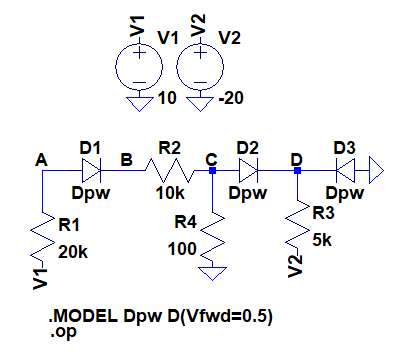
\includegraphics[width=.5\textwidth, height=\textheight, keepaspectratio=true]{ds1b}
\switchcolumn
\begin{tabular}{|l|l|c|}
  \hline  V(a):   &   3.66666        &  voltage
\\\hline  V(v1):  &   10             &  voltage
\\\hline  V(d):   &   -0.500004      &  voltage
\\\hline  V(v2):  &   -20            &  voltage
\\\hline  V(b):   &   3.16666        &  voltage
\\\hline  V(c):   &   -3.2666e-006   &  voltage
\\\hline  I(D3):  &   0.0035833      &  device\_current
\\\hline  I(D2):  &   0.000316699    &  device\_current
\\\hline  I(D1):  &   0.000316667    &  device\_current
\\\hline  I(R4):  &   3.2666e-008    &  device\_current
\\\hline  I(R2):  &   -0.000316667   &  device\_current
\\\hline  I(R3):  &   0.0039         &  device\_current
\\\hline  I(R1):  &   -0.000316667   &  device\_current
\\\hline  I(V2):  &   0.0039         &  device\_current
\\\hline  I(V1):  &   -0.000316667   &  device\_current
\\\hline
\end{tabular}
\end{paracol}
\end{center}

\clearpage
\section{Problem 8.2-5.b.1: } Derived by swapping the independent/dependent state of $P_Z$ and $I_L(\text{max})$ and by changing the values.
\subsection{Design}
Design a voltage regulator using the circuit shown below.
 The voltage regulator is to power a car radio at $V_L = 10 V$ 
 from an automobile battery whose voltage may vary between $14$ and $19 V$. 
 The current in the radio will vary between $0$ (off) to some unknown $I_L(\text{max})$ at full volume.
 The Zener diode has a maximum power rating of $P_Z(\text{max}) = 1W$.
 
\begin{center}
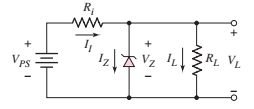
\includegraphics[width=\textwidth, height=7\baselineskip, keepaspectratio=true]{ds2}
\end{center}

\begin{align}
	V_Z 
	  &= V_{\text{radio}} 
	   = 2.5V
\\  I_Z(\text{max}) 
	  &= \frac{P_Z}{V_Z} 
	   = \frac{1W}{10V}
	   = 0.1A
\\  I_Z(\text{max}) 
      &= \frac{
      	I_L(\text{max})[V_{PS}(\text{max}) - V_Z]-I_L(\text{min})[V_{PS}(\text{min})]
      	}{
      	V_{PS}(\text{min}) - 0.9V_Z - 0.1V_{PS}(\text{max})
      	}
\\ \implies 
	I_L(\text{max})
      &= \frac{
      	I_Z(\text{max})
      	[
      	V_{PS}(\text{min}) - 0.9V_Z - 0.1V_{PS}(\text{max})
      	]
      	+
      	I_L(\text{min})[V_{PS}(\text{min})]
      	}{
      	V_{PS}(\text{max}) - V_Z
      	}
\\    &= \frac{
      	0.1A
      	[
      	14V - 0.9\times10V - 0.1\times 19V
      	]
      	}{
      	19V - 10V
      	}
\\    &= 34.44mA
\\  R_i 
      &= \frac{V_{PS}(\text{max})-V_Z}{I_Z(\text{max}) + I_L(\text{min})}
       = \frac{19V - 10V}{0.1A + 0}
       = 90\Omega
\\  P_{R_i}(\text{max}) 
	  &= \frac{(V_{PS}(\text{max}) - V_Z)^2}{R_i}
	   = \frac{(19V - 10V)^2}{90\Omega}
	   = 0.9 W
\\  I_Z(min) 
	  &= \frac{V_{PS}(\text{min}) - V_Z}{R_i} - I_L(\text{max})
	   = \frac{14V-10V}{90\Omega} - 34.44mA
	   = 10mA
\end{align}

\clearpage
\subsection{Validation}

\begin{center}
LTSpice Implementation

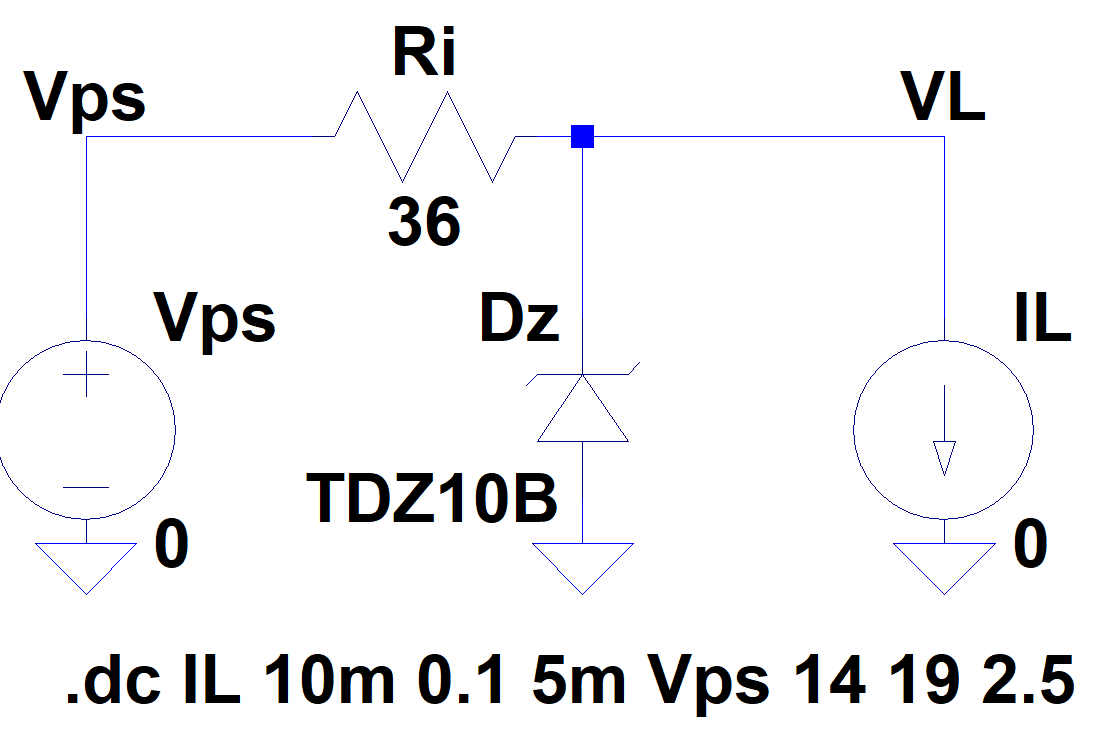
\includegraphics[width=.4\textwidth, height=\textheight, keepaspectratio=true]{ds2b}
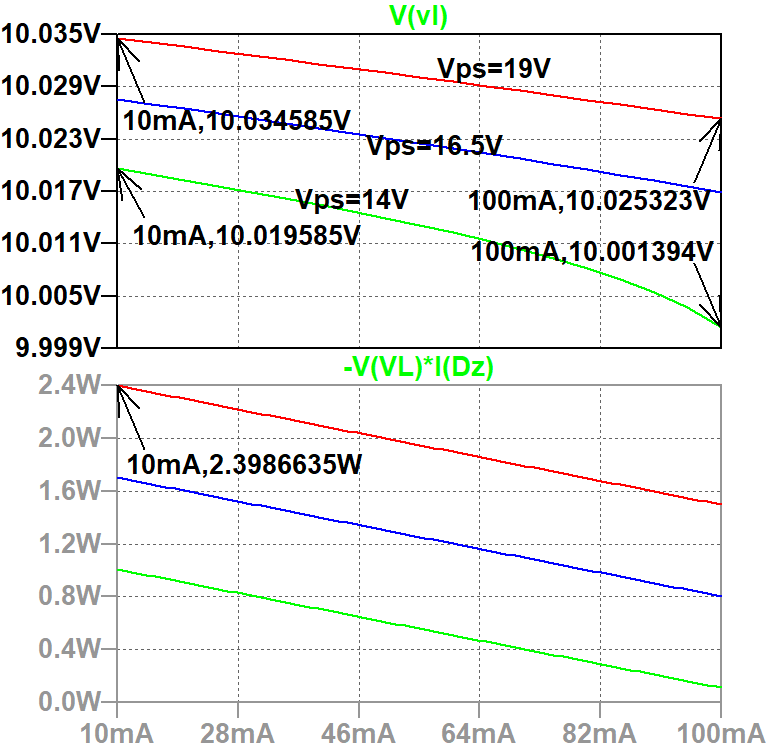
\includegraphics[width=.49\textwidth, height=\textheight, keepaspectratio=true]{ds2c}
$Err_{P} = \frac{|2.5-2.39|}{2.5} = 0.044 = 4.4\%$ High error is due inefficiencies in the circuit.
\end{center}

This assignment should demonstrate a basic understanding of manipulating zener diode voltage regulator circuits and solving multiple diode circuits.

\textit{I have neither given nor received unauthorized assistance on this assignment.}


\end{raggedright}
\end{document}
